\section{Introduction}
\blfootnote{$\dagger$ Work done during an internship at AWS AI Labs.}
\blfootnote{$\ddagger$ Work done while at Amazon.}
Pretrained language models (PTLMs) have achieved remarkable performance on benchmark datasets for a range of NLP tasks~\cite{Liu2019RoBERTaAR, brown2020language}. 
% However, in an open-ended real-world setup, the distribution of data may constantly shift from that of pretraining corpus, 
However, when deployed in the wild, NLP systems must deal with emerging data that have constantly shifting data distribution, different from the text corpora they were initially pretrained on --- for example, when new data domains are introduced (upper part of Fig.~\ref{fig:datasets})~\cite{Gururangan2020DontSP}, or when the language uses and vocabulary change over time (lower part of Fig.~\ref{fig:datasets})~\cite{Lazaridou2021PitfallsOS}. 
% For example, one may extend LMs pretrained on encyclopedia text~\cite{beltagy2019scibert} to new science domains such as biomedical papers. As another example, one may expect PTLMs over Tweets~\cite{nguyen2020bertweet} to continually improve so that it solves tasks over the latest tweets.
%\xiang{should touch on that fine-tuning supposes to help such adaptation but why it may not be sufficient.}
Fine-tuning from a static and possibly ``outdated" PTLM may limit the model performance on downstream tasks, %especially in the low data settings, 
as the PTLM may no longer provide an effective model initialization~\cite{beltagy2019scibert, Mller2020COVIDTwitterBERTAN}.
% data distribution shift makes the static PTLM a suboptimal weight initialization.
% Therefore, we study approaches to continuously adapt PTLMs whenever new corpus become available, while retaining knowledge from corpora seen earlier.
Here we look to understand whether continuously adapting a PTLM to emerging data can yield gains on various downstream tasks, and how to achieve better downstream performance for such lifelong PTLM adaptation.
% Towards this goal, we propose to study lifelong (continual) pretraining of language models: the language model is sequentially pretrained over several corpora without (or with only a little) re-training over previously seen corpora.
%To simulate these challenging scenarios, 
%Therefore, we study lifelong pretraining of language models over a sequence of text corpora in order to adapt the PTLM to the latest corpus while 


\begin{figure}
    \centering
    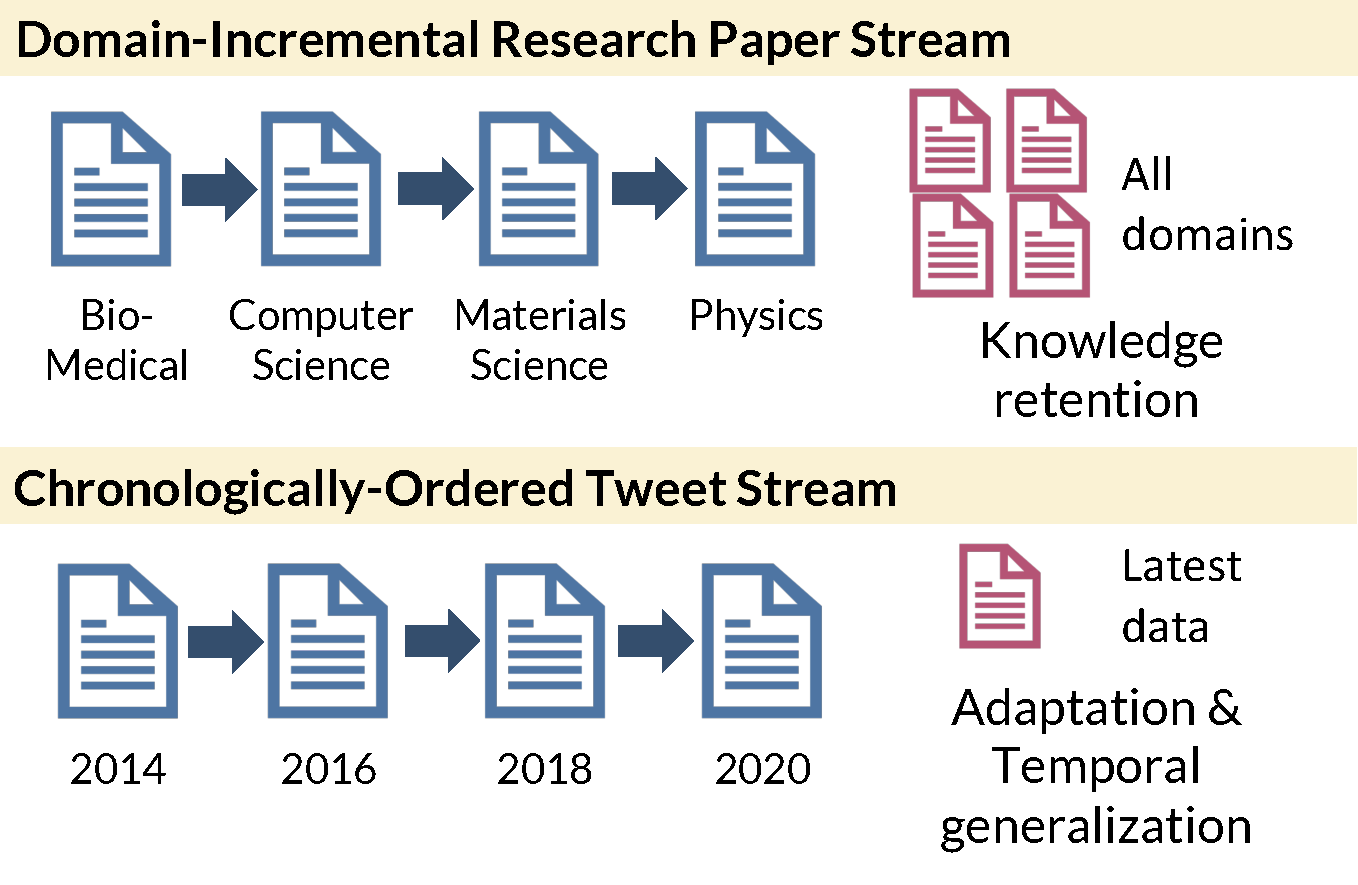
\includegraphics[width=\linewidth]{acl2022/figs/datasets.pdf}
    \caption{Two data streams created for studying lifelong language model pre-training. We focus on evaluating knowledge retention on the domain-incremental research papers stream; we focus on adaptation to the latest data and temporal generalization on the chronologically ordered tweet stream.}
    \label{fig:datasets}
\end{figure}


%\xiang{The current related work paragraph reads a bit vague and weak. I left comments for rewriting.}
A number of recent works make attempts on adapting PTLMs to a new data domain.
\citet{Gururangan2020DontSP, Yao2021AdaptandDistillDS} adapt language models to corpora of different genres and topics
% research papers, news, and product review corpora 
and observe performance improvement in domain-specific downstream tasks.~\citet{Arumae2020AnEI} further show that by regularizing the parameters of PTLMs, the downstream tasks performance on the general domain can be preserved. Another line of works focuses on temporal domain shift~\cite{Hombaiah2021DynamicLM}, which analyzes the effect of pretraining over up-to-date data to the downstream tasks.~\citet{Rttger2021TemporalAO} further study vocabulary composition approaches for improving adaptation to up-to-date corpora.
%In summary, most of existing findings partially address the question on ``\textit{whether adapting PTLMs to a target domain is useful}", through evaluating downstream performance on the target domain. 
However, these work focus their study on adapting PTLM to a single new domain; while in practice, corpora from distinct domains and time stamps may emerge sequentially. 
Whether one can maintain a single, up-to-date PTLM remains an open problem. 
% However, these studies are limited to studying adaptation to only \textit{one} new domain; 
Related to this,~\citet{Lazaridou2021PitfallsOS} study adaptation of PTLMs over temporal data streams, but solely focus on language modeling instead of fine-tuning performance. %investigate the fine-tuning performance on downstream tasks.
% While~\citet{Rttger2021TemporalAO, Hombaiah2021DynamicLM} study the effect of sequential pretraining to downstream tasks, each of them only focuses on a specific metric of success (\textit{e.g.}, downstream performance over latest data). Besides, beyond the analysis, addressing the challenge from a modeling and continual learning perspective has been missing.
It is also important to understand multiple aspects of the utility of lifelong PTLM pretraining, such as knowledge retention over all the seen data, and study what methods can improve the utility of PTLMs in such a continual pretraining process.


%However, continual (sequential) pretraining over multiple distinct corpora is less studied --- it is unclear how the LM can continually acquire and accumulate knowledge from different corpora to benefit downstream tasks in a new domain or on more recent data, and whether the LM can retain the knowledge learned from earlier corpora to preserve decent performance on seen domains. 

% and the forgetting happens to earlier intermediate corpora is less studied.

% While there are abundant prior works on continual learning~\cite{Sun2020LAMOLLM, Kirkpatrick2017OvercomingCF}, 
%\xiang{I think this paragraph needs to be revised and moved after we introduce the analysis workflow and questions (the next paragraph). We can merge this into the method paragraph you currently have, to talk about what are the technical challenges and what methods we examines/compare and how we tweak things to try to resolve the challenges.}
%Furthermore, lifelong LM pretraining poses unique challenges to existing continual learning (CL) methods. 
%For memory-based CL approaches~\cite{Wang2019SentenceEA, chaudhry2019tiny}, a small number of training examples may not be sufficient to represent past knowledge that should be retained, as the size of the pretraining corpus is typically huge. Moreover, there is no guarantee that a CL approach that retains pretraining performance also retains fine-tuning performance well, as the latter solely depends on the learned representations instead of the masked language modeling prediction head. 
% In addition, the focus of evaluation in continual pretraining closely relates to practical use cases: for example, in continual pretraining over multiple text domains, retention of knowledge and less catastrophic forgetting is crucial to the aggregated multi-domain performance; while in continual pretraining over temporal data, it is more crucial how the model performs on the latest data.



In this paper, we formulate a \textit{Lifelong Language Model Pretraining} task to simulate practical scenarios of maintaining and adapting a PTLM over emerging corpora, create a testbed (along with pretraining data streams and downstream tasks) for studying continual pretraining algorithms, and present a systematic evaluation protocol for measuring the progress made on this challenging problem (see Figure~\ref{fig:problem} for an illustration). 
% \xiang{need update.}
We consider two types of text corpus sequences when constructing pretraining data streams, each of which simulates a representative use case and that has slightly different focuses on the evaluation: continuously learning a single model that is applicable to both old and new domains; and improving the model's ability to handle latest data.
%\xiang{needs some rewriting for the below sentence to better clarify the focus and distinctions}
% with major difference in their goals: 
%knowledge retention over all past data, or adaptation to the latest data.
Specifically, we construct
1) a domain-incremental text stream that consists of academic papers published in four research fields, and
2) a temporal tweet stream that consists of tweets collected from four different years.
% Depending on the data stream, 
By conducting systematic experiments on these two data streams,
we look to answer a series of analysis questions: 1) whether continual pretraining retains fine-tuning performance over earlier corpora compared to traditional offline pretraining, 2) whether pretraining improves downstream performance on the latest data, and 3) whether pretraining improves temporal generalization where training and evaluation have distribution gaps because of time.
%\xiang{Expand to include more on the measures of success we're focusing on when answering the above questions -- i.e., what mean good or bad to us?}
%\xiang{Revise to better reflect 1) the ability of PTLMs we look to examine in this task setting; 2) the corresponding analysis questions we asked for the capability above and how we setup the analysis to get answers; and along with 3) the quantitative measurement we focus on for examining the ability.}
%We keep track of the downstream task performance of fine-tuned models and focus on the evaluation of knowledge preservation on the domain-incremental text stream; while for the chronologically ordered stream, we focus on adaptation to latest data and temporal generalization where training and testing distributions are from different time steps in downstream tasks.
%We evaluate fine-tuning performance of downstream tasks selected from earlier works for the research paper stream; while for the tweet stream, we construct downstream datasets using tweets from each year. These downstream datasets allow us to quantify knowledge retention, catastrophic forgetting, and adaption ability of continually pretrained models. 
%\xiang{revise this paragraph a bit to present the analysis questions we look to answer through the experiments.}
%\xiang{say a bit more on the motivation of the following study first.}
%\xiang{Improve this para to 1) smooth out the transition and 2) say more on why this is a non-trivial tech problem and its relation to existing efforts on CL methods (e.g., are existing methods enough? why existing methods may not be effective here;).}
%We further provide extensive analysis on distillation based approaches, integrating various knowledge distillation techniques to continual learning, to dissect the research question - which ``dark knowledge'' should be retained to best improve overall pretraining performance.



%\xiang{Update according based on the analysis questions we asked in earlier paragraph.} % need to be updated based on the latest exp results on twitter
%\xiang{Enrich RE analysis questions above.}
% We try to figure out the best working approach to continually pretrain language models.
To address the research questions above, we conduct a systematic evaluation of existing continual learning (CL) algorithms, spanning over model-expansion based, memory-based, and distillation-based approaches. 
Our results show distillation-based approaches are most effective in knowledge retention in the research paper stream, while simultaneously improve adaptation to latest data and temporal generalization in the tweet stream.
%Our results show that, 1) continual learning algorithms are effective for knowledge retention, where distillation-based approaches perform the best; 2) at the same time, continual pretraining improves adaptation to latest data and temporal generalization.% but does not improve adaptation to latest data on the tweet stream.
We believe our problem formulation, evaluation setup, methods and analysis can inspire more future work on continual pretraining of language models.

